%%%%%%%%%%%%%%%%%%%%%%%%%%%%%%%%%%%%%%%%%%%%%%%%%%%%%%%%%%%%%%%%%
%2345678901234567890123456789012345678901234567890123456789012345
%        1         2         3         4         5         6     
\chapter{Introduction}
\label{cha:introduction}

\section{Background}
\label{sec:background}
\subsection{Non-holonomic omnidirectinal mobile robot}
Mobile robot has been widely used in the industry, like logistics and palletizing, to decrease the dependence on manpower. Among various structrues of mobile robot, omnidirectinal ones are gaining more and more 
importance due to their high maneuverability in the task space, which makes them more flexible and adaptive in complex envirement. The omnidirectinal mobile robots in the market now are mostly equiped with 
Swedish wheel or claster wheel, these kinds of structures are called holonomic omnidirectinal as they have 3 degree of freedom in the joint space w.r.t 3 degree of freedom in the task space. However, their complex 
wheel structure causes a lot of problem in practice, such as vulnerable to uneven ground and noise etc. To avoid such drawback while make use of the flexibility. We put our sight on the so called non-holonomic 
omnidirectinal mobile robot. 

\subsection{Instantaneous Center of Rotation}
\label{sec:Instantaneous Center of Rotation}
To control this kind of robots efficiently without actuator conflict, Instantaneous Center of Rotation(ICR) is always used to moldeling the kinematics. The ICR is defined as being the point in the robot frame that instantaneously does not move in relation to the robot. For our case, the ICR corresponds to the point where the zero motion line of each wheel intersect. This point is time-varying and can be used to analyze the platform state or been controlled in terms of position and velocity to coordinate the wheels to achieve certain twist. 
It's particularly important that the unique existence of ICR corresponds to the fact that the kinematic constraints are respected. And this unique existence of ICR assumption is one of the base of our study.
In practice, we will calculate the desired ICR position/velocity based on the incoming task space command. And estimate the current ICR by the wheel orientations feedback from sensors, which makes it possible for us to do the control on the ICR space with $ICR_{reference}$ and $ICR_{feedback}$. 



\begin{figure}[t]
\begin{center}
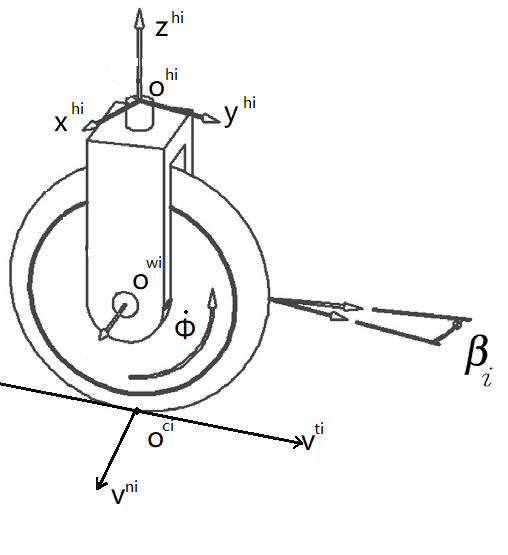
\includegraphics[width=.5\textwidth]{../Figures/wheel.png}
\caption{Wheel structure}
\label{fig:wheel}
\end{center}
\end{figure}
%%%%%%%%%%%%%%%%%%%%%%%%%%%%%%%%%%%%%%%%%%%%%%%%%%%%%%%%%%%%%%%%%%%%%%%%%%%%%%%%%%%%%%%%%%%%%%%%%%%%%%%%%%%%%%%%%%%%%%%%%%%%%%%%%%%%%%%%%%%%%%%%%%%%%%%%%%%%%%%%%%%%%%%%%%%%%%%%%%%%%%%%%%%%%%%%%
%%%%%%%%%%%%%%%%%%%%%%%%%%%%%%%%%%%%%%%%%%%%%%%%%%%%%%%%%%%%%%%%%%%%%%%%%%%%%%%%%%%%%%%%%%%%%%%%%%%%%%%%%%%%%%%%%%%%%%%%%%%%%%%%%%%%%%%%%%%%%%%%%%%%%%%%%%%%%%%%%%%%%%%%%%%%%%%%%%%%%%%%%%%%%%%%%

\section{Problem identification}
\label{sec:problemIdentification}
In the predecessor work, Campion et al. classified all wheeled mobile robots through two feature, degree of mobility$\delta_m$ and degree of steerablity$\delta_s$. $\delta_m$ illustrate the number of dimensions of instantaneously accessible velocity space, while $\delta_s$ resemble the number of independently steerable wheels. Our structure equiped with 4 'Centered orientable wheels'. \textit{centered orientable wheel is such that the motion of the wheel plane with respect to the frame is a rotation around a vertical axle passing through the center of the wheel}\cite{campion1996structural} which is shown in \cref{fig:wheel}. Our platform has four conventional centered orientable wheels, but these wheels need to be coordinate to guarantee a unique ICR as discussed above, The ICR can be define by the intersection of zero motion lines of 2 wheels. Thus there is only 2 independent controllable wheels, and $\delta_s = 2$. From which we can calculate the degree of mobility $\delta_m = 3 - \delta_s = 1$ 

Degree of mobility $\delta_m = 1$ implies that the platform cannot instantaneously change its task space velocity direction. To be able to conduct a task space velocity command, 4 wheels need to be coordinate to a specific
orientation. Such a requirement makes the low-level controller design quite challenging.

There are some strategies proposed before. A typical solution by Sorou et al. \cite{sorour2016kinematic} is to pre-calculate the trajectory so that it is smooth enough and the ICR point through out the trajectory is defined consistently. Such strategies will gurantee a perfect behavior and even could help avoiding singularities in the trajectory. However, in practice, a functional mobile robot need to connect the global planner to be able to interact with the world. Such solution is then not practical. 

When we connect with the global path planner, the incoming task space velocity command from it are usually not smooth w.r.t time, especially when obstacles appear in the way and the trajectory is re-planed. Such problem leads to inconsistent definition of ICR through out the trajectory, as well as inconsistency of steer angle violating the kinematic constraints. Recent study get some  impressing  result by optimizing the ICR position and interpolate it to get feasible smooth trajectory in real-time \cite{sorour2016motion}
However, these solutions still have limitations. Calculating steering angles based on the ICR position make the control frame work not able to handle the simplest case, linear translation, where the ICR is in representation singularity.

%%%%%%%%%%%%%%%%%%%%%%%%%%%%%%%%%%%%%%%%%%%%%%%%%%%%%%%%%%%%%%%%%%%%%%%%%%%%%%%%%%%%%%%%%%%%%%%%%%%%%%%%%%%%%%%%%%%%%%%%%%%%%%%%%%%%%%%%%%%%%%%%%%%%%%%%%%%%%%%%%%%%%%%%%%%%%%%%%%%%%%%%%%%%%%%%%
%%%%%%%%%%%%%%%%%%%%%%%%%%%%%%%%%%%%%%%%%%%%%%%%%%%%%%%%%%%%%%%%%%%%%%%%%%%%%%%%%%%%%%%%%%%%%%%%%%%%%%%%%%%%%%%%%%%%%%%%%%%%%%%%%%%%%%%%%%%%%%%%%%%%%%%%%%%%%%%%%%%%%%%%%%%%%%%%%%%%%%%%%%%%%%%%%
The objective of this paper is to propose a low-level controller framework which is capable of handling the inconsistency trajectory problem. Our work makes use of the achievement from previous study on ICR optimization, while propose a switching control logic to handle the representation singularity problem so that it is capable of handling all circumstance and highly responsive to omnidirectinal velocity commands. 
Thus can be treat as a "real omnidirectinal" structure by the global plannar(navigation)
%%%%%%%%%%%%%%%%%%%%%%%%%%%%%%%%%%%%%%%%%%%%%%%%%%%%%%%%%%%%%%%%%%%%%%%%%%%%%%%%%%%%%%%%%%%%%%%%%%%%%%%%%%%%%%%%%%%%%%%%%%%%%%%%%%%%%%%%%%%%%%%%%%%%%%%%%%%%%%%%%%%%%%%%%%%%%%%%%%%%%%%%%%%%%%%%%
%%%%%%%%%%%%%%%%%%%%%%%%%%%%%%%%%%%%%%%%%%%%%%%%%%%%%%%%%%%%%%%%%%%%%%%%%%%%%%%%%%%%%%%%%%%%%%%%%%%%%%%%%%%%%%%%%%%%%%%%%%%%%%%%%%%%%%%%%%%%%%%%%%%%%%%%%%%%%%%%%%%%%%%%%%%%%%%%%%%%%%%%%%%%%%%%%

The remainder of this thesis is organized as follows.
\cref{cha:Kinematic} illustrate how do we derive the forward and inverse kinematic model.
\cref{cha:framework} introduce the mobile robot platform structure, the implementation details, the two control strategies and how do we switch between them.
\cref{cha:ICR} detailed explained the ICR optimization control strategy.
\cref{cha:inverseKinematics} detailed explained the inverse kinematic approximation control strategy.
The experiment result is discussed in \cref{cha:experiment}.